Neste capítulo apresentaremos fatos básicos da teoria de superfícies no espaço Euclidiano $\R^3$ e na esfera $\Sp^3$. Teremos como base as referências \cite{Carmo1987}, \cite{Meeks2012}, \cite{Nitsche2011}, \cite{Brendle2013} e \cite{Dajczer2019}.

\section{Subvariedades em formas espaciais}

Nesta seção apresentaremos, sem demonstrações, as equações fundamentais de uma imersão isométrica entre duas variedades Riemannianas dando enfoque, em especial, quando o espaço ambiente é uma forma espacial. Admitiremos conhecidos todos os pré-requisitos de Geometria Riemanniana necessários à compreensão dessa seção.

Dadas duas variedades Riemannianas $M^m$ e $\tilde{M}^n$, uma \emph{imersão isométrica} entre $M$ e $\tilde{M}$ é uma aplicação diferenciável $f: M \rightarrow \tilde{M}$ que é uma imersão e, para todo $p \in M$, satisfaz
\begin{equation}\label{def-imersao}
\innerproduct{X}{Y} = \innerproduct{df(p) X}{df(p) Y},	
\end{equation}
para quaisquer $X,Y \in T_p M$. A diferença $n-m$ é chamada a \emph{codimensão} de $f$. Observe que se $f: M \rightarrow \tilde{M}$ é uma imersão e $\innerproduct{}{}$ é uma métrica em $\tilde{M}$, a condição \eqref{def-imersao} define uma métrica em $M$, a \emph{métrica induzida} por $f$, que torna $f$ uma imersão isométrica.

\begin{definicao}
	Dada uma imersão isométrica $f: M \rightarrow \tilde{M}$, seja $f^* T \tilde{M}$ o fibrado induzido sobre $M$, cuja fibra em $p \in M$ é $T_{f(p)} \tilde{M}$. O complemento ortogonal de $f_* T_p M$ em $T_{f(p)} \tilde{M}$, denotado por $T_p M^\perp$, chama-se o \emph{espaço normal} de $f$ em $p$. O \emph{fibrado normal} $TM^\perp$ de $f$ é o subfibrado vetorial de $f^* T \tilde{M}$, cuja fibra em $p \in M$ é $T_p M^\perp$.
\end{definicao}

A conexão de Levi-Civita $\tilde{\nabla}$ de $\tilde{M}$ induz uma única conexão $\hat{\nabla}$ em $f^* T \tilde{M}$ tal que
\[ \hat{\nabla}_X (Z \circ f) = \tilde{\nabla}_{f_* X} Z, \]
para quaisquer $X \in \vectorfieldsspace{M}$ e $Z \in \vectorfieldsspace{\tilde{M}}$. Identificaremos sempre $\hat{\nabla}$ com $\tilde{\nabla}$.

Dados dois campos vetoriais $X,Y \in \vectorfieldsspace{M}$, decompomos
\[ \tilde{\nabla}_X f_* Y = \parenthesis{\tilde{\nabla}_X f_* Y}^\top + \parenthesis{\tilde{\nabla}_X f_* Y}^\perp, \]
com relação à decomposição ortogonal
\[ f^* T \tilde{M} = f_* TM \oplus TM^\perp. \]
A aplicação
\[ \nabla_X Y = f_*^{-1} \parenthesis{\tilde{\nabla}_X f_* Y}^\top \]
define uma conexão compatível e sem torção em $TM$, logo coincide com a conexão de Levi-Civita de $M$.

\begin{definicao}
	A aplicação $\alpha_f: \vectorfieldsspace{M} \times \vectorfieldsspace{M} \rightarrow \Gamma \parenthesis{TM^\perp}$ definida por
	\[ \alpha_f (X,Y) = \parenthesis{\tilde{\nabla}_X f_* Y}^\perp \]
	chama-se a \emph{segunda forma fundamental} da imersão isométrica $f$.
\end{definicao}

Obtemos, assim, a fórmula de Gauss
\[ \tilde{\nabla}_X f_* Y = f_* \nabla_X Y + \alpha_f (X,Y), \]
para quaisquer $X, Y \in \vectorfieldsspace{M}$.

\begin{observacao}
	Como
	\[ \tilde{\nabla}_X f_* Y - \tilde{\nabla}_Y f_* X = f_* [X,Y], \]
	para quaisquer $X.Y \in \vectorfieldsspace{M}$, segue que
	\[ \alpha_f (X,Y) - \alpha_f(Y,X) = f_* [X,Y] - f_* [X,Y] = 0, \]
	ou seja, $\alpha_f$ é simétrica. Além disso, $\alpha_f$ é $\smoothfunctionsspace{M}$-bilinear, o valor de $\alpha_f (X,Y)$ em $p \in M$ depende somente dos valores dos campos $X$ e $Y$ em $p$.
\end{observacao}

O \emph{operador de forma} $A_\xi$ de $f$ em relação a um campo vetorial $\xi \in \Gamma \parenthesis{TM^\perp}$ é definido por
\[ \innerproduct{A_\xi X}{Y} = \innerproduct{\alpha_f (X,Y)}{\xi}, \]
para quaisquer $X,Y \in \vectorfieldsspace{M}$. Dados $X,Y \in \vectorfieldsspace{M}$ e $\xi \in \Gamma \parenthesis{TM^\perp}$, temos:
\begin{align*}
	\innerproduct{\tilde{\nabla}_X \xi}{f_* Y} &= - \innerproduct{\xi}{\tilde{\nabla}_X f_* Y}\\
	&= -\innerproduct{\xi}{\alpha_f (X,Y)}\\
	&= -\innerproduct{A_\xi X}{Y}.
\end{align*}
Assim,
\[ \parenthesis{\tilde{\nabla}_X \xi}^\top  = -f_* A_\xi X. \]
Além disso, a componente normal
\[ \nabla^\perp_X \xi = \parenthesis{\tilde{\nabla}_X \xi}^\perp \]
define uma conexão compatível em $TM^\perp$, chamada a \emph{conexão normal} de $f$. Obtemos, assim, a \emph{fórmula de Weingarten}
\[ \tilde{\nabla}_X \xi = - f_* A_\xi X + \nabla^\perp_X \xi. \]

\begin{definicao}
	O \emph{vetor curvatura média} de $f$ no ponto $p \in M$ é o vetor normal
	\begin{equation}\label{def-curvatura-media}
		H(p) = \frac{1}{m} \sum_{i=1}^{m} \alpha_f (X_i, X_i),
	\end{equation}
	onde $\{ X_1, \ldots, X_m \}$ é uma base ortonormal de $T_p M$. Segue de \eqref{def-curvatura-media} que
	\begin{align*}
		m \innerproduct{H}{\xi} &= \sum_{i=1}^{m} \innerproduct{\alpha_f (X_i, X_i)}{\xi} = \sum_{i=1}^{m} \innerproduct{A_\xi X_i}{X_i}\\
		&= \tr A_\xi,
	\end{align*}
	logo o lado direito de \eqref{def-curvatura-media} não depende da escolha da base ortonormal.
\end{definicao}

\begin{definicao}
	Uma imersão isométrica $f: M \rightarrow \tilde{M}$ é dita \emph{mínima num ponto} $p \in M$ se $H(p)=0$. Diremos que $f$ é \emph{mínima} se for mínima em todos os pontos $p \in M$.
\end{definicao}

Usando as fórmulas de Gauss e Weingarten, podemos obter as equações de compatibilidade para uma dada imersão isométrica $f: M^m \rightarrow \tilde{M}^n$. De forma mais precisa, as equações de Gauss, Codazzi e Ricci para a imersão isométrica $f$ são dadas, respectivamente, por
\begin{gather}\label{eq-gauss}
	\innerproduct{R(X,Y)Z}{W} = \innerproduct{\tilde{R}(X,Y)Z}{W} + \innerproduct{\alpha_f (X,W)}{\alpha_f(Y,Z)} - \innerproduct{\alpha_f (X,Z)}{\alpha_f (Y,W)},\\
	\label{eq-codazzi}
	\parenthesis{\tilde{R}(X,Y)Z}^\perp = \parenthesis{\nabla^\perp_X \alpha_f}(Y,Z) - \parenthesis{\nabla^\perp_Y \alpha_f}(X,Z)
\end{gather}
e
\begin{equation}\label{eq-ricci}
	\innerproduct{R^\perp (X,Y) \xi}{\eta} = \innerproduct{\tilde{R}(X,Y) \xi}{\eta} + \innerproduct{[A_\xi, A_\eta] X}{Y},
\end{equation}
para quaisquer $X,Y,Z,W \in \vectorfieldsspace{M}$ e $\xi, \eta \in \Gamma \parenthesis{TM^\perp}$.

Quando $\tilde{M}^n$ denota uma variedade Riemanniana de curvatura seccional constante igual a $c$, as equações \eqref{eq-gauss}, \eqref{eq-codazzi} e \eqref{eq-ricci} tornam-se, respectivamente
\begin{gather}\label{eq-gauss-em-formas-espaciais}
\innerproduct{R(X,Y)Z}{W} = c \innerproduct{\parenthesis{X \wedge Y} Z}{W} + \innerproduct{\alpha_f (X,W)}{\alpha_f(Y,Z)} - \innerproduct{\alpha_f (X,Z)}{\alpha_f (Y,W)},\\
\label{eq-codazzi-em-formas-espaciais}
\parenthesis{\nabla^\perp_X \alpha_f}(Y,Z) = \parenthesis{\nabla^\perp_Y \alpha_f}(X,Z)
\end{gather}
e
\begin{equation}\label{eq-ricci-em-formas-espaciais}
\innerproduct{R^\perp (X,Y) \xi}{\eta} = \innerproduct{[A_\xi, A_\eta] X}{Y}.
\end{equation}

Seja $\mathbb{Q}^n_c$ uma forma espacial completa, simplesmente conexa e com curvatura seccional constante $c$. Para os espaços ambientes $\mathbb{Q}^n_c$, as equações de compatibilidade \eqref{eq-gauss-em-formas-espaciais}, \eqref{eq-codazzi-em-formas-espaciais} e \eqref{eq-ricci-em-formas-espaciais} são equações intrínsecas relacionando o tensor de curvatura de $M^m$, a segunda forma fundamental de $f$ e o tensor de curvatura da conexão normal. Assim, é natural se perguntar se tais dados, satisfazendo as equações de compatibilidade de um fibrado vetorial sobre uma variedade Riemanniana $M^m$ podem ser realizados como os dados associados com uma imersão isométrica de $M^m$ em $\mathbb{Q}^n_c$.

O \emph{teorema fundamental para subvariedades} (cf. \cite[Theorem 1.10]{Dajczer2019}) estabelece que isso é, localmente, sempre verdadeiro, e também globalmente quando $M^m$ é simplesmente conexa. Além disso, independente do fato de $M^m$ ser simplesmente conexa, a imersão isométrica é única a menos de isometrias do espaço ambiente.

No caso particular de uma hipersuperfície $f: M^n \rightarrow \mathbb{Q}^{n+1}_c$, as equações fundamentais tornam-se somente duas. Mais precisamente, as equações de Gauss e Codazzi para $f$ podem ser expressas como sendo
\begin{equation}
	R(X,Y)Z = c \parenthesis{X \wedge Y} Z + \parenthesis{AX \wedge AY} Z
\end{equation}
e
\begin{equation}
	\parenthesis{\nabla_Y A} X = \parenthesis{\nabla_X A} Y,
\end{equation}
respectivamente.

No caso mais particular de uma superfície $f: M^2 \rightarrow \mathbb{Q}^3_c$, imersa numa forma espacial tridimensional, a curvatura seccional da superfície $M^2$ em $\mathbb{Q}^3_c$, munida da métrica induzida, coincide com sua curvatura Gaussiana, a menos da constante $c$. De forma mais precisa, a curvatura Gaussiana intrínseca $K_{\text{int}}$ de $M^2$ é dada por
\begin{equation}\label{eq:gausshyp}
	K_{\text{int}} = K_{\text{ext}} + c,
\end{equation}
onde $K_{\text{ext}}$ denota a curvatura extrínseca de $M^2$, que é dada pelo produto das curvaturas principais de $M^2$.


\section{Superfícies mínimas em $\realnumbers^3$}

Uma superfície regular $M$ em $\R^3$ é dita ser uma \emph{superfície mínima} se sua curvatura média $H$ é nula em todos os pontos. O plano é, trivialmente, uma superfície mínima, pois suas curvaturas principais são identicamente nulas em todos os pontos.

Antes de estudarmos mais exemplos, faremos algumas considerações. Seja $M \subset \R^3$ uma superfície orientada e considere uma função diferenciável $f: M \rightarrow \R$. Uma \emph{variação normal} de $M$ dada por $f$ é uma família de superfícies $M_t$, com $t \in (-\epsilon,\epsilon)$, dadas por
\begin{equation*}
	p_t = p + t f(p) N(p),
\end{equation*}
onde $N$ é o campo unitário, normal a $M$, na orientação positiva de $M$. Para $\epsilon > 0$ suficientemente pequeno, cada $M_t$ é uma superfície regular, chamada uma \emph{superfície de variação}. Note que, para $t=0$ tem-se $M_0 = M$, e que se $f \equiv 1$, $M_t$ é uma \emph{superfície paralela} a $M$ a uma distância $t$.

Dados uma variação normal $M_t$ de $M$, relativa a uma função diferenciável $f: M \rightarrow \R$, com $t \in (-\epsilon,\epsilon)$, e um domínio limitado $D \subset M$, considere o conjunto
\begin{equation*}
	D_t = \left\{ p_t \in M_t: p \in D \right\},
\end{equation*}
com $t \in (-\epsilon,\epsilon)$. Para cada instante $t \in (-\epsilon,\epsilon)$, o conjunto $D_t$ é o domínio correspondente em $M_t$. Definimos, para cada $t \in (-\epsilon,\epsilon)$,
\begin{equation*}
	A(t) = \text{Área} (D_t).
\end{equation*}
Vale o seguinte resultado, cuja demonstração pode ser encontrada em \cite{Nitsche2011}:

\begin{teorema}
	Nas condições acima, vale
	\begin{equation}\label{primeira-variacao-da-area}
		A'(0) = -2 \int_D H f dA,
	\end{equation}
	onde $dA$ denota o elemento de área de $M$.
\end{teorema}

A fórmula \eqref{primeira-variacao-da-area} é conhecida como \emph{primeira variação da área}. Como consequência, temos a seguinte:

\begin{proposicao}\label{superficie-minima-como-ponto-critico-do-funcional-da-area}
	Uma superfície $M$ em $\R^3$ é mínima se, e somente se, $A'(0)=0$.
\end{proposicao}

\begin{demonstracao}
	Se $M$ é uma superfície mínima, então $H \equiv 0$, logo segue de \eqref{primeira-variacao-da-area} que $A'(0)=0$. Reciprocamente, suponha $A'(0)=0$ para toda função diferenciável $f: M \rightarrow \R$. Suponha que existe um ponto $p \in M$ tal que $H(p)>0$. Podemos escolher $f$ tal que $f(p) = H(p)$, $f \geq 0$ e $f \equiv 0$ no complementar de um domínio $D$ de $M$, com $p \in D$ e $H \vert_D >0$. Para uma tal função $f$, temos
	\begin{equation*}
		A'(0) = -\int_M H f dA <0,
	\end{equation*}
	o que é uma contradição. Portanto, deve-se ter $H(p)=0$, para todo $p \in M$.
\end{demonstracao}

A palavra mínima, neste contexto, está relacionada com o seguinte problema proposto por Lagrange em 1760: dado uma curva fechada $\gamma$ em $\R^3$, sem auto-interseções, determinar a superfície de área mínima que tem $\gamma$ como fronteira.

Suponha que exista uma solução $M$ para o problema de Lagrange, e considere uma variação normal $M_t$ de $M$, com $t \in (-\epsilon,\epsilon)$, dada por uma função diferenciável $f: M \rightarrow \R$, com $f \vert_{\partial M} \equiv 0$. Como a área de $M$ é mínima tem-se, em particular, que
\begin{equation*}
	A(t) \geq A(0),
\end{equation*}
para todo $t \in (-\epsilon,\epsilon)$ e toda tal variação. Portanto, $A'(0)=0$ qualquer que seja a função $f: M \rightarrow \R$, com $f \vert_{\partial M} \equiv 0$. Isso mostra, em virtude da Proposição \ref{superficie-minima-como-ponto-critico-do-funcional-da-area}, que as superfícies de área mínima são superfícies mínimas no sentido da definição usual. A recíproca, no entanto, é falsa.

\begin{proposicao}
	Não existem superfícies mínimas e compactas em $\R^3$.
\end{proposicao}

\begin{demonstracao}
	Se $M$ é uma superfície mínima em $\R^3$, então
	\begin{equation*}
		H = \frac{1}{2} (k_1 + k_2) = 0.
	\end{equation*}
	Isso implica que $k_1=-k_2$ em todos os pontos de $M$, logo a curvatura Gaussiana $K$ satisfaz $K = k_1 k_2 \leq 0$. No entanto, toda superfície compacta em $\R^3$ admite um ponto $p$ tal que $K(p)>0$, e isso nos dá uma contradição.
\end{demonstracao}

Dado uma superfície regular $M$ em $\realnumbers^3$, considere uma carta local isotérmica $(U,\varphi)$ para $M$, i.e., 
\begin{equation*}
E = G = \lambda^2 \text{ e } F=0,
\end{equation*}
onde $\lambda: U \rightarrow \realnumbers$ é uma função diferenciável, com $\lambda > 0$. Note que, nas coordenadas isotérmicas $\varphi \sim (x,y)$, a curvatura média $H$ se expressa como
\begin{equation*}
H = \frac{e + g}{2 \lambda^2}.
\end{equation*}

\begin{definicao}
	Dado uma função diferenciável $f: U \subset \realnumbers^2 \rightarrow \realnumbers$, o \emph{Laplaciano} de $f$, denotado por $\Delta f$, é definido por
	\begin{equation*}
	\Delta f = \frac{\partial^2 f}{\partial x^2} + \frac{\partial^2 f}{\partial y^2}.
	\end{equation*}
	Dizemos que $f$ é \emph{harmônica} se $\Delta f = 0$.
	
	Se $(U, \varphi)$ é uma carta local para $M$, como $\varphi = (\varphi_1, \varphi_2, \varphi_3)$, definimos
	\begin{equation*}
	\Delta \varphi = (\Delta \varphi_1, \Delta \varphi_2, \Delta \varphi_3).
	\end{equation*}
\end{definicao}

\begin{proposicao}
	Se $(U, \varphi)$ é uma carta local isotérmica em $M$, então 
	\begin{equation*}
	\Delta \varphi = 2 \lambda^2 H N.
	\end{equation*}
\end{proposicao}

\begin{demonstracao}
	Como $\varphi$ é isotérmica, com $\varphi \sim (u, v)$, temos
	\begin{equation*}
	\innerproduct{\varphi_u}{\varphi_v} = \lambda^2 = \innerproduct{\varphi_v}{\varphi_u} \quad \text{e} \quad \innerproduct{\varphi_u}{\varphi_v} = 0.
	\end{equation*}
	Derivando, obtemos:
	\begin{equation*}
	\innerproduct{\varphi_{uu}}{\varphi_u} = \innerproduct{\varphi_{vu}}{\varphi_v} = - \innerproduct{\varphi_u}{\varphi_{vv}}.
	\end{equation*}
	Disso decorre que
	\begin{equation}\label{eq1}
	\innerproduct{\varphi_{uu} + \varphi_{vv}}{\varphi_u} = 0.
	\end{equation}
	Analogamente, obtemos:
	\begin{equation}\label{eq2}
	\innerproduct{\varphi_{uu} + \varphi_{vv}}{\varphi_v} = 0.
	\end{equation}
	De \eqref{eq1} e \eqref{eq2} concluímos que $\varphi_{uu} + \varphi_{vv}$ é paralela a $N$. Além disso, como
	\begin{equation}
	H = \frac{e+g}{2 \lambda^2},
	\end{equation}
	obtemos
	\begin{equation*}
		2 \lambda^2 H = e + g = \innerproduct{\varphi_{uu} + \varphi_{vv}}{N},
	\end{equation*}
	mostrando que
	\begin{equation}
	\Delta \varphi = 2 \lambda^2 H N,
	\end{equation}
	como queríamos.
\end{demonstracao}

\begin{corolario}\label{equiv_isoterma_harmonica}
	Uma superfície $M$ em $\realnumbers^3$ é mínima se, e somente se, toda carta local isotérmica é harmônica.
\end{corolario}

\begin{exemplo}
	O \emph{catenóide} é a superfície em $\realnumbers^3$ gerada pela rotação da catenária 
	\begin{equation*}
	y = a \cosh \left( \frac{z}{a} \right)
	\end{equation*}
	em torno do eixo-$z$.
	Assim, o catenóide pode ser parametrizado por
	\begin{equation*}
	\varphi(u,v) = \left( a \cosh v \cos u, a \cosh v \sin u, av \right),
	\end{equation*}
	onde $u \in (0, 2 \pi)$ e $v \in \realnumbers$. Para tal $\varphi$, obtemos
	\begin{equation*}
	E = G = a^2 \cosh^2 v, \quad F = 0 \quad \text{e} \quad \varphi_{uu} + \varphi_{vv} = 0.
	\end{equation*}
	Portanto o catenóide é uma superfície mínima.
\end{exemplo}

\begin{figure}
	\centering
	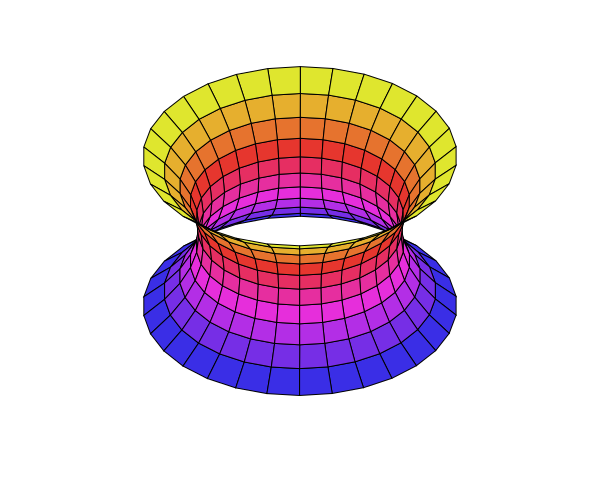
\includegraphics[width=0.5\textwidth]{images/catenoid}
	\caption{Catenóide. Autor: Matthias Weber. Creative Commons Attribution-Noncommercial-No Derivative Works 3.0 Unported License (\url{http://creativecommons.org/licenses/by-nc-nd/3.0/}). Enlace: \url{https://minimal.sitehost.iu.edu/archive/Classical/Classical/Catenoid/web/index.html}}
\end{figure}

\begin{exemplo}
	Considere uma hélice dada por
	\begin{equation*}
	\alpha(u) = \left( \cos u, \sin u, au \right).
	\end{equation*}
	Por cada ponto da hélice, trace uma reta paralela ao plano-$xy$ que intercepta o eixo-$z$ ortogonalmente.
	A superfície gerada por tais retas é o \emph{helicóide} e pode ser parametrizada por
	\begin{equation*}
	\varphi(u,v) = \left( v \cos u, v \sin u, au \right),
	\end{equation*}
	com $u \in (0, 2 \pi)$ e $v \in \realnumbers$. Temos
	\begin{equation*}
	E = G = a^2 \cosh^2 v, \quad F = 0 \quad \text{e} \quad \varphi_{uu} + \varphi_{vv} = 0.
	\end{equation*}
	Portanto o helicóide é uma superfície mínima.
\end{exemplo}

\begin{figure}
	\centering
	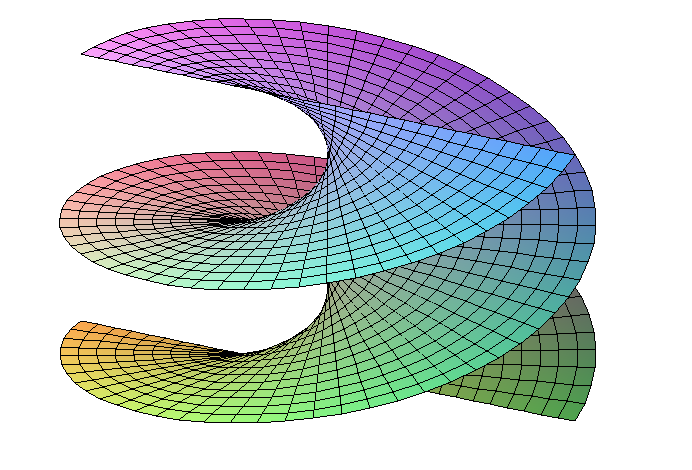
\includegraphics[width=0.5\textwidth]{images/helicoid}
	\caption{Helicóide. Autor: Matthias Weber. Creative Commons Attribution-Noncommercial-No Derivative Works 3.0 Unported License (\url{http://creativecommons.org/licenses/by-nc-nd/3.0/}). Enlace: \url{https://minimal.sitehost.iu.edu/archive/Classical/Classical/Helicoid/web/index.html}}
\end{figure}

\begin{teorema}
	Além do plano,
	\begin{enumerate}
		\item[a)] O catenóide é a única superfície rotacional mínima.
		\item[b)] O helicóide é a única superfície regrada mínima.
	\end{enumerate}
\end{teorema}

\begin{demonstracao}
	Para a demonstração de $a)$, ver \cite[§3.5, Exemplo 5]{Carmo2010}. 
	Para a demonstração de $b)$, ver \cite[§3.5, Exemplo 6]{Carmo2010}.
\end{demonstracao}

\begin{exemplo}
	Dado uma função diferenciável $f: U \rightarrow \realnumbers$, definida num aberto $U \subset \realnumbers^2$, considere o gráfico $\text{Gr}(f)$ de $f$, parametrizado por
	\begin{equation*}
	\varphi(x,y) = (x,y,f(x,y)), \quad (x,y) \in U.
	\end{equation*}
	Temos
	\begin{align*}
	\varphi_x &= (1,0,f_x),\\
	\varphi_y &= (0,1,f_y).
	\end{align*}
	Assim
	\begin{align*}
	E &= \innerproduct{\varphi_x}{\varphi_x} = 1 + f_x^2,\\
	F &= \innerproduct{\varphi_x}{\varphi_y} = f_x f_y,\\
	G &= \innerproduct{\varphi_y}{\varphi_y} = 1 + f_y^2.
	\end{align*}
	Um campo $n$, normal a $\text{Gr}(f)$, é dado por
	\begin{equation*}
	n = \varphi_x \times \varphi_y = \det \left[ \begin{matrix}
	i & j & k\\
	1 & 0 & f_x\\
	0 & 1 & f_y
	\end{matrix} \right]\\
	= (-f_x, -f_y, 1).
	\end{equation*}
	Normalizando, temos
	\begin{equation*}
	N = \frac{n}{\norm{n}} = \frac{1}{\sqrt{1 + f_x^2 + f_y^2}}(-f_x, -f_y, 1).
	\end{equation*}
	Como
	\begin{align*}
	\varphi_{xx} &= (0, 0, f_{xx})\\
	\varphi_{xy} &= (0, 0, f_{xy})\\
	\varphi_{yy} &= (0, 0, f_{yy})
	\end{align*}
	obtemos
	\begin{align*}
	e &= \innerproduct{\varphi_{xx}}{N} = \frac{f_{xx}}{\sqrt{1 + f_x^2 + f_y^2}},\\
	f &= \innerproduct{\varphi_{xy}}{N} = \frac{f_{xy}}{\sqrt{1 + f_x^2 + f_y^2}},\\
	g &= \innerproduct{\varphi_{yy}}{N} = \frac{f_{yy}}{\sqrt{1 + f_x^2 + f_y^2}}.
	\end{align*}
	Assim, como
	\begin{equation*}
	H = \frac{eG - 2fF + gE}{2(EG - F^2)}
	\end{equation*}
	segue que $H \equiv 0$ se, e somente se,
	\begin{equation}\label{edp_superficies_minimas}
	(1 + f_y^2) f_{xx}  - 2 f_x f_y f_{xy} + (1+f_x^2) f_{yy} = 0,
	\end{equation}
	que é uma EDP de 2\textsuperscript{a} ordem.
	Uma solução simples da equação \eqref{edp_superficies_minimas} é a função linear
	\begin{equation*}
	f(x,y) = ax + by + c,
	\end{equation*}
	como $a, b, c \in \realnumbers$.
\end{exemplo}

\begin{exemplo}[Superfície de Scherk]
	Considere uma função $f$ dada por
	\begin{equation*}
	f(x,y) = g(x) + h(y),
	\end{equation*}
	onde  $g(x,y)=g(x)$ e $h(x,y)=h(y)$. Neste caso, a equação \eqref{edp_superficies_minimas} pode ser escrita como
	\begin{equation*}
	(1 + (h')^2(y)) g''(x) + (1 + (g')^2(x)) h''(y) = 0,
	\end{equation*}
	ou seja,
	\begin{equation*}
	\frac{g''(x)}{1 + (g')^2(x)} + \frac{h''(y)}{1 + (h')^2(y)} = 0.
	\end{equation*}
	Isso implica
	\begin{equation*}
	\frac{g''(x)}{1 + (g')^2(x)} = - \frac{h''(y)}{1 + (h')^2(y)} = \text{constante}.
	\end{equation*}
	Integrando, obtemos (a menos de constantes) que
	\begin{equation*}
	g(x) = \ln (\cos x) \quad \text{e} \quad h(y) = -\ln (\cos y).
	\end{equation*}
	A menos de dilatações e translações, uma parte da superfície pode ser representada pelo gráfico da função
	\begin{equation*}
	\ln \left( \frac{\cos x}{\cos y} \right), \quad 0 < x,y < \frac{\pi}{2}.
	\end{equation*}
\end{exemplo}

\begin{figure}
	\centering
	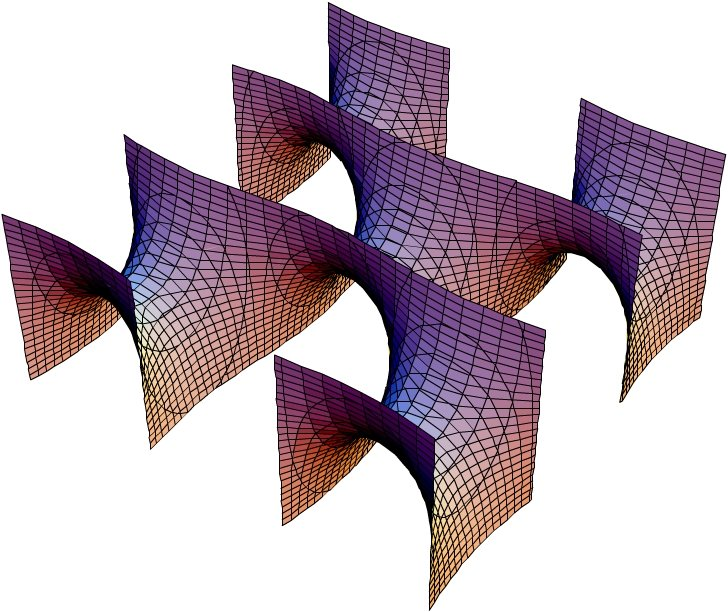
\includegraphics[width=0.5\textwidth]{images/scherk}
	\caption{Superfície de Scherk. Autor: Matthias Weber. Creative Commons Attribution-Noncommercial-No Derivative Works 3.0 Unported License (\url{http://creativecommons.org/licenses/by-nc-nd/3.0/}). Enlace: \url{https://minimal.sitehost.iu.edu/archive/Classical/Classical/SinglyScherk/web/index.html}}
\end{figure}

\section{A fórmula de representação de Weierstrass}
Nesta seção apresentaremos a fórmula de representação de Weierstrass que tem como objetivo gerar superfícies mínimas em $\R^3$. Esta fórmula faz uso da teoria de superfícies de Riemann e Análise Complexa.

Considere o plano complexo $\complexnumbers$ identificado com $\realnumbers^2$ através da aplicação injetora 
\begin{equation*}
(x,y) \in \realnumbers^2 \mapsto x + iy \in \complexnumbers.
\end{equation*}
Uma função complexa $f: U \subset \complexnumbers \rightarrow \complexnumbers$ pode ser escrita na forma
\begin{equation*}
f(u,v) = f_1(u,v) + i f_2(u,v),
\end{equation*}
onde $f_1, f_2: U \rightarrow \realnumbers$ são funções reais, denotadas por
\begin{align*}
f_1 &= \Re(f)\\
f_2 &= \Im(f)
\end{align*}
tal que $\Re(f)$ é parte real da função $f$ e $\Im(f)$ é a parte imaginaria da função $f$.
\begin{definicao}
	Uma função $f: U \subset \complexnumbers \rightarrow \complexnumbers$, definida no aberto $U$, é dita \emph{holomorfa} se $f_1, f_2$ possuem derivadas parciais contínuas e satisfazem as equações de Cauchy-Riemann
	\begin{equation*}
		\begin{split}
		\partialdifffrac{f_1}{u} &= \partialdifffrac{f_2}{v}\\
		\partialdifffrac{f_1}{v} &= - \partialdifffrac{f_2}{u}
		\end{split}.
	\end{equation*}

\end{definicao}

Dados uma superfície $M \subset \realnumbers^3$ e uma carta local $(U, \varphi)$ em $M$, com
\begin{equation*}
\varphi(u,v) = (x_1(u,v), x_2(u,v), x_3(u,v)),
\end{equation*}
considere as funções complexas $f_j: U \subset \complexnumbers \rightarrow \complexnumbers, 1 \leq j \leq 3,$ dadas por
\begin{equation}\label{carta_isoterma_cauchy-riemann}
f_j = \partialdifffrac{x_j}{u} - i \partialdifffrac{x_j}{v}, \quad 1 \leq j \leq 3.
\end{equation}

\begin{lema}
	Seja $(U, \varphi)$ uma carta local isotérmica em $M$. Então, $\varphi$ é mínima se, e somente se, cada $f_j$, definida em \eqref{carta_isoterma_cauchy-riemann}, é holomorfa.
\end{lema}

\begin{demonstracao}
	Pelo Corolário \ref{equiv_isoterma_harmonica}, temos que $\varphi$ é mínima se, e somente se, $\varphi$ é harmônica, i.e., $\varphi_{uu} + \varphi_{vv} = 0$. Isso significa que
	\begin{equation*}
	\npartialdifffrac{x_j}{u}{2} + \npartialdifffrac{x_j}{v}{2} = 0, \quad 1 \leq j \leq 3.
	\end{equation*}
	Queremos provar que
	\begin{align*}
	\pdiff{u} \Re(f_j) &= \pdiff{v} \Im(f_j),\\
	\pdiff{v} \Re(f_J) &= - \pdiff{u} \Im(f_j).
	\end{align*}
	Assim
	\begin{equation*}
	\pdiff{u} \Re(f_J) = \pdiff{u} \partialdifffrac{x_j}{u} = \npartialdifffrac{x_j}{u}{2} = - \npartialdifffrac{x_j}{v}{2} = \pdiff{v} \left( - \partialdifffrac{x_j}{v} \right) = \pdiff{v} \Im(f_j).
	\end{equation*}
	Isso prova a primeira equação de Cauchy-Riemann. Por outro lado, como a superfície é regular, vale
	\begin{equation*}
	\varphi_{uv} = \varphi_{vu},
	\end{equation*}
	ou seja
	\begin{equation*}
	\frac{\partial^2 x_j}{\partial u \partial v} = \frac{\partial^2 x_j}{\partial v \partial u}.
	\end{equation*}
	Assim
	\begin{equation*}
	\pdiff{v} \Re(f_j) = \pdiff{v} \partialdifffrac{x_j}{u} = \pdiff{u} \partialdifffrac{x_j}{v}
	= \pdiff{u} \left( - \Im(f_j) \right)
	= - \pdiff{u} \Im(f_j),
	\end{equation*}
	que é a segunda equação de Cauchy-Riemann.
\end{demonstracao}

\begin{lema}\label{lema_fj_2}
	Sejam $M \subset \realnumbers^3$ uma superfície mínima e $(U, \varphi)$ uma carta local isotérmica. Então, as funções holomorfas $f_j$, definidas em \eqref{carta_isoterma_cauchy-riemann}, satisfazem
	\begin{gather}\label{sum_fj_2}
	f_1^2 + f_2^2 + f_3^2 = 0\\ \label{sum_norm_fj_2}
	|f_1|^2 + |f_2|^2 + |f_3|^2 \neq 0.
	\end{gather}
	Reciprocamente, sejam $f_1, f_2, f_3$ funções holomorfas, definidas num aberto simplesmente conexo $U \subset \complexnumbers$, satisfazendo \eqref{sum_fj_2} e \eqref{sum_norm_fj_2}. Então, tais funções dão origem a uma carta local isotérmica mínima $(U, \varphi)$, cujas funções coordenadas satisfazem \eqref{carta_isoterma_cauchy-riemann}.
\end{lema}

\begin{demonstracao}
	Seja $(U, \varphi)$ uma carta local isotérmica em $M$. Então,
	\begin{align*}
	f_1^2 + f_2^2 + f_3^2 &= \sum_{j=1}^{3} \left[ \left( \partialdifffrac{x_j}{u} \right)^2 - \left( \partialdifffrac{x_j}{v} \right)^2 - 2i \partialdifffrac{x_j}{u} \partialdifffrac{x_j}{v} \right]\\
	&= E - G - 2iF = 0,
	\end{align*}
	pois $E=G$ e $F=0$. A equação \eqref{sum_norm_fj_2} segue da regularidade de $\varphi$, pois $\varphi_u \neq 0$ e $\varphi_v \neq 0$.
	Reciprocamente, defina
	\begin{equation}\label{carta_isoterma_eq_integral}
	x_j(u,v) = \int_{\xi_0}^{\xi} f_j(z) dz, \quad 1 \leq j \leq 3
	\end{equation}
	com $\xi = (u,v) \in U$, para algum $\xi_0 \in U$ fixado. Note que cada $x_j$ está bem definida, pois $U$ é simplesmente conexo e $f_j$ é holomorfa, o que nos dá uma função holomorfa definida em $U$, para qual podemos aplicar as equações de Cauchy-Riemann, obtendo:
	\begin{align*}
	\frac{d}{d \xi} \int_{\xi_0}^{\xi} f_j &= \frac{d}{d \xi} \left[ \Re \int_{\xi_0}^{\xi} f_j + i \Im \int_{\xi_0}^{\xi} f_j \right]\\
	&= \pdiff{u} \Re \int_{\xi_0}^{\xi} f_j + i \pdiff{u} \Im \int_{\xi_0}^{\xi} f_j\\
	&= \pdiff{u} \Re \int_{\xi_0}^{\xi} f_j - i \pdiff{v} \Re \int_{\xi_0}^{\xi} f_j,
	\end{align*}
	de modo que a equação \eqref{carta_isoterma_cauchy-riemann} é válida. Considere a aplicação $\varphi: U \rightarrow \realnumbers^3$, cujas funções coordenadas
	\begin{equation*}
	\varphi = (x_1,x_2,x_3)
	\end{equation*}
	são dadas como em \eqref{carta_isoterma_eq_integral}. De \eqref{sum_fj_2} e \eqref{sum_norm_fj_2} segue que $(U,\varphi)$ é uma carta local isotérmica. Além disso, as funções $f_j$ serem holomorfas implica que as funções coordenadas $x_j$ são harmônicas, logo, pelo Corolário \ref{equiv_isoterma_harmonica}, $\varphi$ é mínima.
\end{demonstracao}

\begin{observacao}
	As funções $x_j$ definidas em \eqref{carta_isoterma_eq_integral} estão definidas a menos de uma constante aditiva, de modo que a superfície está definida a menos de uma translação. Assim, o estudo local de superfícies mínimas em $\realnumbers^3$ reduz-se a resolver as equações \eqref{sum_fj_2} e \eqref{sum_norm_fj_2} para uma terna de funções holomorfas.
\end{observacao}

\begin{teorema}\label{teorema-de-representacao-de-weierstrass}
	Sejam $f: U \subset \complexnumbers \rightarrow \complexnumbers$ uma função holomorfa e $g: U \rightarrow \complexnumbers$ uma função meromorfa tais que $fg^2$ seja holomorfa. Assuma que se $\xi \in U$ é um polo de ordem $n$ para $g$ então $\xi$ é um zero para $f$ de ordem $2n$, e que estes sejam os únicos zeros de $f$.
	Então, a aplicação
	\begin{equation}\label{carta_minima_duas_funcoes}
	\varphi(z) = \frac{1}{2} f(z) \left( (1-g(z)^2), i (1+g(z)^2), 2g(z) \right)
	\end{equation}
	satisfaz as condições do Lema \ref{lema_fj_2}. Além disso, para toda tal $\varphi$, existem funções holomorfa $f$ e meromorfa $g$ tais que vale \eqref{carta_minima_duas_funcoes}.
\end{teorema}

\begin{demonstracao}
	Se $\varphi$ satisfaz \eqref{carta_minima_duas_funcoes}, temos
	\begin{align*}
	f_1^2 + f_2^2 + f_3^2 &= \frac{1}{4} f(z)^2 (1 - g(z)^2)^2 - \frac{1}{4} f(z)^2 (1 + g(z)^2)^2 + f(z)^2 g(z)^2\\
	&= -f(z)^2 g(z)^2 + f(z)^2 g(z)^2 =0.
	\end{align*}
	Afirmamos que $\varphi(z) \neq 0, \forall z \in U$. De fato, a hipótese sobre os zeros de $f$ e os polos de $g$ implica que $f(z) g(z)^2 \neq 0$. Assim, para qualquer $z$ fixado, a primeira e a segunda coordenadas de $\varphi$ não podem ser ambas nulas.
	Assim, podemos assumir que $\varphi$ é holomorfa satisfazendo
	\begin{equation*}
	\varphi_1^2 + \varphi_2^2 + \varphi_3^2 \not\equiv 0,
	\end{equation*}
	$\varphi$ nunca é zero, e considere
	\begin{equation*}
	f(z) = \varphi_1(z) - i \varphi_2(z) \quad \text{e} \quad
	g(z) = \frac{\varphi_3(z)}{\varphi_1(z) - i \varphi_2(z)}.
	\end{equation*}
	$f$ é uma função holomorfa e $g$ é o quociente de funções holomorfas. Se o denominador de $g$ é identicamente nulo, fazemos
	\begin{equation*}
	g(z) = \frac{\varphi_3(z)}{\varphi_1(z) + i \varphi_2(z)}
	\end{equation*}
	e procedemos de forma similar.
	Assim, sendo o denominador de $g$ não nulo, tem-se que $g$ é meromorfa. Logo, a relação
	\begin{equation*}
	\varphi_1^2 + \varphi_2^2 + \varphi_3^2 = 0
	\end{equation*}
	implica
	\begin{equation*}
	(\varphi_1 + i \varphi_2)(\varphi_1 - i \varphi_2) = -\varphi_3^2
	\end{equation*}
	que, em termos de $f$ e $g$, torna-se
	\begin{align*}
	\varphi_1 + i \varphi_2 &= \frac{-\varphi_3^2}{\varphi_1 - i \varphi_2}\\
	&= \frac{-\varphi_3^2}{(\varphi_1 - i \varphi_2)^2} (\varphi_1 - i \varphi_2)\\
	&= -fg^2
	\end{align*}
	Esta última equação, juntamente com as condições sobre $f$ e $g$, nos dão $\varphi$ como em \eqref{carta_minima_duas_funcoes}.
\end{demonstracao}

\begin{definicao}
	Sejam $U \subset \complexnumbers$ um aberto simplesmente conexo e $\gamma \subset U$ uma curva de um ponto fixado $z_0 \in U$ a um ponto arbitrário $z \in U$, $z = u + iv$.
	Sejam $f,g$ como no Teorema \ref{teorema-de-representacao-de-weierstrass}. Então,
	\begin{equation*}
	\varphi(u,v) = (x_1(u,v), x_2(u,v), x_3(u,v)),
	\end{equation*}
	onde
	\begin{align*}
	x_1 &= \Re \int_{\gamma} \frac{1}{2} f(z) (1 - g(z)^2) dz\\
	x_2 &= \Re \int_{\gamma} \frac{1}{2} f(z) (1 + g(z)^2) dz\\
	x_3 &= \Re \int_{\gamma} f(z) g(z) dz
	\end{align*}
	é uma carta local mínima, chamada \emph{a representação de Weierstrass} da teoria local de superfícies mínimas.
\end{definicao}

\begin{exemplo}[Catenóide]
	O catenóide pode ser representado pelas funções holomorfas $f, g: \complexnumbers \rightarrow \complexnumbers$ dadas por
	\begin{equation*}
	f(z) = e^{-z} \quad \text{e} \quad
	g(z) = e^z.
	\end{equation*}
	Substituindo tais funções na fórmula da representação de Weierstrass, e integrando de $z_0 = 0$ a um ponto arbitrário $z = u + iv$, obtemos
	\begin{align*}
	\varphi(u,v) &= x_0 + \Re \int_{z_0}^{z} \frac{f(\xi)}{2} (1 - g(\xi)^2, i (1 + g(\xi)^2), 2 g(\xi)) d\xi\\
	&= x_0 + \Re \int_{z_0}^{z} \frac{e^{-\xi}}{2} (1 - e^{2\xi}, i (1 + e^{2\xi}), 2e^{\xi}) d\xi\\
	&= \Re \int_{0}^{z} \frac{1}{2} (e^{-\xi} - e^{\xi}, i (e^{-\xi} + e^{\xi}), 1) d\xi\\
	&= \Re \left[ \frac{1}{2} \left(-e^{-z} - e^z, -\frac{1}{2i} (-e^{-z} + e^z), z \right) \right] \\
	&= \Re \left( -\cosh z, i \sinh z, z \right) \\
	&= \left( -\cosh u \cos v, -\cosh u \sin v, u \right).
	\end{align*} 
\end{exemplo}

\begin{exemplo}[Superfície de Enneper]
	A superfície de Enneper pode ser representada pelas funções holomorfas $f,g: \complexnumbers \rightarrow \complexnumbers$ dadas por
	\begin{equation*}
	f(z) = 1 \quad \text{e} \quad
	g(z) = z.
	\end{equation*}
	Assim, a representação de Weierstrass torna-se
	\begin{align*}
	\varphi(u,v) &= \Re \left( \frac{1}{2} \int_{0}^{z} \left( 1 - \xi^2, i (1 + \xi^2), 2\xi \right) \right) d\xi \\
	&= \frac{1}{2} \Re \left( z - \frac{z^3}{3}, iz + \frac{iz^3}{3}, z^2 \right) \\
	&= \frac{1}{2} \left( u - \frac{u^3}{3} + uv^2, -v + \frac{v^3}{3} - u^2v, u^2 - v^2 \right).
	\end{align*}
\end{exemplo}

\begin{figure}
	\centering
	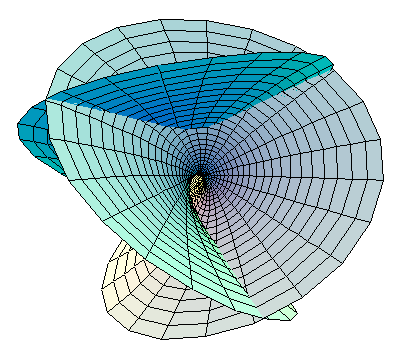
\includegraphics[width=0.5\textwidth]{images/enneper}
	\caption{Superfície de Enneper. Autor: Matthias Weber. Creative Commons Attribution-Noncommercial-No Derivative Works 3.0 Unported License (\url{http://creativecommons.org/licenses/by-nc-nd/3.0/}). Enlace: \url{https://minimal.sitehost.iu.edu/archive/Classical/Classical/Enneper/web/index.html}}
\end{figure}

\begin{exemplo}[Superfície de Scherk]
	A superfície de Scherk, definida pela equação
	\begin{equation*}
	e^z = \frac{\cos y}{\cos x},
	\end{equation*}
	pode ser representada pelas funções holomorfas $f: \complexnumbers \setminus \{\pm 1, \pm i \} \rightarrow \complexnumbers$ e $g: \complexnumbers \rightarrow \complexnumbers$ dadas por
	\begin{equation*}
	f(z) = \frac{2}{1 - z^4} \quad \text{e} \quad
	g(z) = z.
	\end{equation*}
	Note que
	\begin{align*}
	f (1 - g^2) &= \frac{2}{1 + z^2} = \frac{i}{z + i} - \frac{i}{z - i}, \\
	i f (1 + g^2) &= \frac{2i}{1 - z^2} = \frac{i}{z + 1} - \frac{i}{z - 1}, \\
	2fg &= \frac{4z}{1 - z^4} = \frac{2z}{z^2 + 1} - \frac{2z}{z^2 - 1}.
	\end{align*}
	Assim, substituindo na representação de Weierstrass e integrando, obtemos
	\begin{equation*}
	\varphi(z) = \left( -\arg \frac{z + i}{z - i}, -\arg \frac{z + i}{z - i}, \log \left\| \frac{z^2 + 1}{z^2 - 1} \right\| \right).
	\end{equation*}
	Usando as identidades
	\begin{align*}
	\frac{z + i}{z - i} &= \frac{|z|^2 - 1}{|z^2 - i|^2} + i \frac{z + \overline{z}}{|z - i|^2}, \\
	\frac{z + 1}{z - 1} &= \frac{|z|^2 - 1}{|z - 1|^2} + i \frac{\overline{z} - z}{|z - 1|^2},
	\end{align*}
	podemos encontrar as expressões para $\cos x$ e $\cos y$. Temos
	\begin{align*}
	\cos x &= \cos \left( -\arg \frac{z + i}{z - i} \right) \\
	&= \cos \left( \arg \frac{z + i}{z - i} \right) \\
	&= \cos \left( \arg \left( \frac{|z - i|}{|z + i|} \frac{z + i}{z - i} \right) \right) \\
	&= \Re \left( \frac{|z - i|}{|z + i|} \frac{z + i}{z - i} \right) \\
	&= \frac{|z - i|}{|z + i|} \Re \left( \frac{z + i}{z - i} \right) \\
	&= \frac{|z - i|}{|z + i|} \frac{|z|^2 - 1}{|z - i|^2} = \frac{|z|^2 - 1}{|z^2 + 1|}.
	\end{align*}
	Analogamente, temos
	\begin{align*}
	\cos y &= \cos \left( -\arg \frac{z + 1}{z - 1} \right) \\
	&= \frac{|z - 1|}{|z + 1|} \frac{|z|^2 - i}{|z - 1|^2} \\
	&= \frac{|z|^2 - i}{|z^2 - 1|}
	\end{align*}
	Isso implica que
	\begin{equation*}
	\frac{\cos y}{\cos x} = \frac{z^2 + 1}{|z^2 - 1|} = e^z.
	\end{equation*}
	
	Vejamos uma aplicação da representação de Weierstrass. Dado uma superfície mínima $M \subset \realnumbers^3$, seja $(U, \varphi)$ uma carta local isotérmica.
	Isso significa que
	\begin{equation*}
	E = G = \lambda^2 \quad \text{e} \quad
	F = 0,
	\end{equation*}
	onde
	\begin{align*}
	\lambda^2 &= \frac{1}{2} \sum_{j=1}^{3} |f_j|^2 \\
	&= \frac{1}{4} |f|^2 |1 + g|^2 + \frac{1}{4} |f|^2 |1 + g|^2 + |fg|^2\\
	&= \left( \frac{|f| (| + |g|^2)}{2} \right)^2.
	\end{align*} 
	Além disso, temos
	\begin{align*}
	\varphi_u \times \varphi_v &= \left( \Im (f_2 \overline{f}_3), \Im (f_3 \overline{f}_1), \Im (f_1 \overline{f}_2) \right) \\
	&= \frac{|f|^2 (1 + |g|^2)}{4} \left( 2 \Re(g), 2 \Im(g), |g|^2 - | \right)\\
	\quad \text{e} \quad \| \varphi_u \times \varphi_v \| &= \sqrt{EG - F^2} = \lambda^2,
	\end{align*}
	de modo que
	\begin{equation*}
	N = \left( \frac{2 \Re(g)}{|g|^2 + 1}, \frac{2 \Im(g)}{|g|^2 + 1}, \frac{|g|^2 - 1}{|g|^2 + 1} \right).
	\end{equation*}
	Lembremos que a projeção estereográfica
	\begin{equation*}
	\pi: S^2 \setminus \{ (0,0,1) \} \rightarrow \complexnumbers
	\end{equation*}
	é a aplicação dada por
	\begin{equation*}
	\pi(x_1, x_2, x_3) = \frac{x_1 + ix_2}{1 - x_3},
	\end{equation*}
	e sua inversa é dada por
	\begin{equation*}
	\pi^{-1}(z) = \left( \frac{2 \Re(z)}{|z|^2 + 1}, \frac{2 \Im(z)}{|z|^2 + 1}, \frac{|z|^2 - 1}{|z|^2 + 1} \right).
	\end{equation*}
	Portanto, temos que
	\begin{equation}\label{eq:projecao-esterografica}
	N = \pi^{-1} \circ g.
	\end{equation}
	Podemos resumir isso no seguinte resultado.
\end{exemplo}

\begin{proposicao}
	Sejam $M \subset \realnumbers^3$ uma superfície mínima e $(U, \varphi)$ uma carta local isotérmica. Então, um dos campos unitários $N$, normal a $M$ é a inversa da projeção estereográfica da função $g$ dada pela representação de Weierstrass.
\end{proposicao}

%\begin{teorema}[Teorema de Bernstein]
%	Seja $M \subset \realnumbers^3$ uma superfície mínima definida no plano todo. Então, ou $M$ é um plano.
%%	 ou a imagem da aplicação de Gauss omite pelo menos dois pontos.
%\end{teorema}

%\begin{demonstracao}
%	Se $M$ não está contida num plano, podemos construir a função $g$ que é meromorfa no plano todo $\complexnumbers$. Pelo teorema de Picard, ela atinge todos seus valores com, pelo menos, duas exceções, ou $g$ é constante. A equação \eqref{eq:projecao-esterografica} mostra que o mesmo se aplica a $N$ e, no último caso, $M$ está contida num plano.
%\end{demonstracao}

\begin{teorema}[Existência local de parâmetros isotérmicos]
	Seja $M \subset \realnumbers^3$ uma superfície mínima. Então, todo $p \in M$ pertence a uma vizinhança coordenada isotérmica.
\end{teorema}

\begin{demonstracao}
	Seja $U \subset M$ uma vizinhança coordenada de $p$ que é o gráfico de uma função diferenciável que podemos assumir ser da forma $z = h(x,y), (x,y) \in U$.
	Lembrando que a equação para gráficos mínimos \eqref{edp_superficies_minimas}  é dada por
	\begin{equation*}
	(1 + h_y^2) h_{xx} - 2 h_x h_y h_{xy} + (1 + h_x^2) h_{yy} = 0,
	\end{equation*}
	obtemos a equação
	\begin{equation*}
	\pdiff{x} \frac{1 + h_y^2}{W} = \pdiff{y} \frac{h_x h_y}{W}
	\end{equation*}
	em $U$, onde $W = \sqrt{1 + h_x^2 + h_y^2}$. Escolhendo $U$ simplesmente conexo, isso implica que existe uma função diferenciável $\phi: U \rightarrow \realnumbers$, com
	\begin{equation*}
	\partialdifffrac{\phi}{x} = \frac{h_x h_y}{W} \quad \text{e} \quad
	\partialdifffrac{\phi}{y} = \frac{1 + h_y^2}{W}.
	\end{equation*}
	Introduza novas coordenadas
	\begin{equation*}
	\overline{x} = x \quad \text{e} \quad
	\overline{y} = \phi(x,y).
	\end{equation*}
	Um cálculo simples mostra que
	\begin{align*}
	\partialdifffrac{x}{\overline{x}} &= 1, \\
	\partialdifffrac{x}{\overline{y}} &= 0, \\
	\partialdifffrac{y}{\overline{x}} &= -\frac{h_x h_y}{1 + h_y^2}, \\
	\partialdifffrac{y}{\overline{y}} &= \frac{W}{1 + h_y^2},
	\end{align*}
	e os coeficientes da segunda forma fundamental, em relação a $(\overline{x}, \overline{y})$, são
	\begin{equation*}
	E = G = \frac{W^2}{1 + h_y^2} \quad \text{e} \quad
	F = 0,
	\end{equation*}
	como queríamos.
\end{demonstracao}

\section{Superfícies mínimas em $\Sp^3$}

Nesta seção apresentaremos alguns resultados básicos sobre superfícies mínimas na esfera $\Sp^3$. Indicaremos as referências onde as demonstrações podem ser encontradas. Discutiremos também a minimalidade do toro de Clifford.

A esfera unitária $\Sp^3$ é a hipersuperfície de $\R^4$ dada por
\[ \Sp^3 = \{ x \in \R^4: x_1^2 + x_2^2 + x_3^2 + x_4^2 = 1. \} \]
Dado uma superfície $M$ em $\Sp^3$, seja $\nu$ um campo vetorial unitário, normal ao longo de $M$. Isso significa que $\nu$ é tangente à esfera $\Sp^3$ e, para cada ponto $p \in M$, tem-se $\nu(p) \in T_p M^\perp$. Decorre da equação de Gauss \eqref{eq:gausshyp} para a superfície $M$ em $\Sp^3$ que a curvatura Gaussiana intrínseca $K$ de $M$ é dada por
\[ K = \lambda_1 \lambda_2 + 1, \]
onde $\lambda_1$ e $\lambda_2$ são as curvaturas principais do operador de forma de $M$ associado ao campo normal $\nu$.

Assim como para superfícies em $\R^3$, a soma das curvaturas principais será denotada como a curvatura média de $M$
\[ H = \lambda_1 + \lambda_2 = \sum_{i=1}^{2} \innerproduct{\tilde{\nabla}_{X_i} \nu}{X_i}, \]
onde $\{X_1,X_2\}$ é um referencial local tangente a $M$ e $\tilde{\nabla}$ denota a conexão de Levi-Civita de $\Sp^3$. A curvatura média de $M$ pode ser interpretada, geometricamente, como um $L^2$-gradiente do funcional de área. De forma mais precisa, dada qualquer função $\varphi \in \smoothfunctionsspace{M}$, tem-se
\[ \frac{d}{dt} \text{Área} (M_t) \vert_{t=0} = \int_M H \varphi, \]
onde
\[ M_t = \{ \cos(t \varphi(x))x + \sin(t \varphi(x) N(x)): x \in M \}. \]

Analogamente ao caso Euclidiano, essa interpretação variacional motiva a definir uma superfície na esfera $\Sp^3$ como sendo \emph{mínima} se sua curvatura média $H$ for identicamente nula. O conceito de minimalidade em $\Sp^3$ pode ser formulado de várias formas equivalentes (cf. \cite[Theorem 3.2.1]{Simons1968} e \cite{Dajczer2019}).

\begin{teorema}\label{propriedades_sup_min_S3}
	Dada uma superfície $M$ em $\Sp^3$, as seguintes afirmações são equivalentes:
	\begin{enumerate}
		\item[a)] $M$ é uma superfície mínima.
		\item[b)] $M$ é um ponto crítico do funcional área.
		\item[c)] As restrições das funções coordenadas em $\R^4$ são autofunções do operador Laplaciano $-\Delta_M$ com autovalor igual a 2, ou seja, $\Delta_M x_i = -2 x_i$, com $1 \leq i \leq 4$.
	\end{enumerate}
\end{teorema}

Ao contrário do que ocorre em $\R^3$, de que não existem superfícies mínimas fechadas, existem exemplos interessantes desse fenômeno em $\Sp^3$. Um exemplo simples de superfície mínima fechada em $\Sp^3$ é o equador, que é definido por
\[ M = \{ x \in \Sp^3 \subset \R^4: x_4=0 \}. \]
Neste caso, as curvaturas principais são ambas iguais a zero, logo o equador é uma superfície mínima. Além disso, o equador tem curvatura Gaussiana constante igual a 1. Assim, munido da métrica induzida, $M$ é isométrico à esfera usual $\Sp^2$.

Vejamos outro exemplo importante.

\begin{exemplo}[toro de Clifford]
	Considere a aplicação $x: \R^2 \rightarrow \R^4$ definida por
	\begin{equation}\label{def:toro-de-clifford}
		x(u,v) = \frac{1}{\sqrt{2}} \parenthesis{\cos u, \sin u, \cos v, \sin v}.
	\end{equation}
	Claramente $x$ é uma aplicação diferenciável e tem-se
	\[ \frac{\partial x}{\partial u} = \frac{1}{\sqrt{2}} \parenthesis{-\sin u, \cos u, 0, 0} \]
	e
	\[ \frac{\partial x}{\partial v} = \frac{1}{\sqrt{2}} \parenthesis{0,0, -\sin v, \cos v}. \]
	Disso decorre, em particular, que $x$ é uma imersão. Além disso, como 
	\[x(u + 2k \pi, v + 2l \pi) = x(u,v), \] 
	para quaisquer $(u,v) \in \R^2$ e $k,l \in \mathbb{Z}$, segue que a imagem $x(\R^2)$ é um toro $\Sp_{\sqrt{2}}^1 \times \Sp_{\sqrt{2}}^1 \subset \R^4$. A fim de entender a geometria deste toro, fixemos o seguinte referencial ortonormal
	\begin{align*}
		e_1 &= \parenthesis{-\sin u, \cos u, 0, 0},\\
		e_2 &= \parenthesis{0, 0, -\sin v, \cos v},\\
		e_3 &= \frac{1}{\sqrt{2}} \parenthesis{\cos u, \sin u, \cos v, \sin v},\\
		e_4 &= \frac{1}{\sqrt{2}} \parenthesis{-\cos u, -\sin u, \cos v, \sin v}.
	\end{align*}
	Observe que o vetor posição $e_3 = x$ descreve uma esfera unitária, pois $\norm{x} = 1$. Assim, o toro $x(\R^2)$ está contido na esfera unitária $\Sp^3 \subset \R^4$. Além disso, o referencial $\{e_1,e_2,e_4\}$ é tangente a $\Sp^3$, com
	$e_4$ normal ao toro $x(\R^2)$. Como imersão isométrica, $x: \Sp_{\sqrt{2}}^1 \times \Sp_{\sqrt{2}}^1 \rightarrow \Sp^3$ é conhecida como o \emph{toro de Clifford}. Denotemos por $(h_{ij})$ a matriz da segunda forma fundamental do toro em relação ao campo normal $e_4$. Cada entrada da matriz é dada por
	\begin{equation*}
		\begin{split}
			h_{11} &= \innerproduct{A e_1}{e_1}\\
			h_{12} &= \innerproduct{A e_1}{e_2}\\
			h_{21} &= \innerproduct{A e_2}{e_1}\\
			h_{22} &= \innerproduct{A e_2}{e_2}
		\end{split},
	\end{equation*}
	onde $AX$ é dado por
	\[ AX = -\tilde{\nabla}_X e_4, \]
	para qualquer vetor tangente $X$ ao toro $x(\R^2)$. Temos:
	\begin{align*}
		A e_1 &= -\tilde{\nabla}_{\frac{\partial}{\partial u}} e_4 = \frac{1}{\sqrt{2}} \parenthesis{-\sin u, \cos u, 0, 0},\\
		A e_2 &= -\tilde{\nabla}_{\frac{\partial}{\partial v}} = \frac{1}{\sqrt{2}} \parenthesis{0,0, \sin v, -\cos v}.
	\end{align*}
	Substituindo, obtemos:
	\[ h_{11} = \frac{1}{\sqrt{2}}, \qquad h_{12}=h_{21}=0 \qquad \text{e} \qquad h_{22} = -\frac{1}{\sqrt{2}}. \]
	Disso decorre, em particular, que as curvaturas principais do toro $x(\R^2)$ são $\lambda_1 = \frac{1}{\sqrt{2}}$ e $\lambda_2 = -\frac{1}{\sqrt{2}}$, ou seja, o toro de Clifford é uma superfície mínima.
\end{exemplo}

\begin{observacao}
	Reparametrizando a aplicação dada em \eqref{def:toro-de-clifford}, as curvaturas principais do toro de Clifford podem ser reobtidas como sendo $\lambda_1=1$ e $\lambda_2=-1$. Decorre então da equação de Gauss \eqref{eq:gausshyp} que a curvatura Gaussiana intrínseca do toro de Clifford é nula, ou seja, é uma superfície flat na esfera $\Sp^3$.
\end{observacao}

%A prova de este resultado depende de resultados importantes que serão mencionados a continuação.
%\begin{teorema}\label{thm:takahashi}
%	Se uma imersão isométrica $x: M \rightarrow \R^{m+k}$ de uma $m$-variedade riemanniana em o $(m+k)$-espaço euclideano satisfaz $ \Delta x = \lambda x $ para alguma constante $\neq 0$, então $\lambda$ é necessariamente positiva e $x$ é uma imersão mínima em a esfera $S^{m+k-1}$ de radio $\sqrt{m/\lambda}$ em $\R^{m+k}$. De igual forma, se $x$ é uma imersão mínima em uma esfera de radio $a$ em $\R^{m+k}$, então $x$ satisfaz $\Delta x = \lambda x$ salvo um deslocamento paralelo em $\R^{m+k}$ e $\lambda = m/a^2$.
%\end{teorema}

%\begin{demonstracao}
%	Ver \cite[Theorem 3]{TAKAHASHI1966}.
%\end{demonstracao}

%\begin{definicao}
%	Seja $M$ uma variedade $p$-dimensional, $\tilde{M}$ uma variedade $n$-dimensional, e $f: M \rightarrow \tilde{M}$ uma imersão de $M$ en $\tilde{M}$.
%	Seja $\{ f_t \}$ uma família de imersões uniparamétricas de $M \rightarrow \tilde{M}$ com a propriedade que $f_0 = f$, e seja a função $F: M \times [0,1] \rightarrow \tilde{M}$, definida por $F(m,t) = f_t(m)$, $C^{\infty}$. Então $\{ f_t \}$ é chamado de \emph{a variação de f}.
%\end{definicao}

%\begin{teorema}\label{thm:minimo-e-compacto-implica-ser-ponto-minimo-do-funcional-de-area}
%	Seja $M$ uma variedade $p$-dimensional, $\tilde{M}$ uma variedade $n$-dimensional, e $f: M \rightarrow \tilde{M}$ uma imersão de $M$ en $\tilde{M}$ como variedade mínima.
%	Seja $\{ f_t \}$ uma variação de $f$. Supor que para todo $t$, $ f_t(\partial M) = f(\partial M) $. Então se $M$ é compacto e $\mathcal{A}(t) =$ área de $M$ baixo $f_t$, $\mathcal{A}'(0)=0$.
%\end{teorema}

%\begin{demonstracao}
%	Ver \cite[Theorem 3.2.1]{Simons1968}.
%\end{demonstracao}



%\begin{demonstracao}[Prova do teorema \ref{propriedades_sup_min_S3}]
%	Pelo teorema \ref{thm:takahashi} tem-se a equivalência entre $a)$ e $c)$. Pelo teorema \ref{thm:minimo-e-compacto-implica-ser-ponto-minimo-do-funcional-de-area} tem-se que $a)$ implica $b)$. Para ver a prova de que $b)$ implica $a)$ ir a \cite[\S 2.4]{Simons1968}.
%\end{demonstracao}

%\begin{definicao}
%	O \emph{equador} é um subconjunto de $\Sp^3$ definido por:
%	\begin{equation}
%	M = \left\{ x \in \Sp^3: x_4 = 0 \right\}
%	\end{equation}
%\end{definicao}

%\begin{proposicao}
%	As curvaturas principais do equador são nulas.
%\end{proposicao}

%\begin{demonstracao}
%	É claro que o campo de vetores normais unitários é constante e é dado pelo vetor $(0,0,0,1)$. Portanto a diferencial do campo é nulo e as curvaturas são nulas.
%\end{demonstracao}

%\begin{corolario}
%	O equador é uma superfície mínima em $\Sp^3$.
%\end{corolario}

%\begin{demonstracao}
%	Como a equação da curvatura media em $\Sp^3$ está dada pela soma das curvaturas principais, então, pela proposição anterior, a curvatura media é nula. Portanto é uma superfície mínima.
%\end{demonstracao}

%\subsection{Quantas superfícies mínimas compactas mergulhadas em $\Sp^3$ existem?}

%Por muito tempo o equador e o toro de Clifford eram os únicos exemplos de superfícies mínimas mergulhadas em $\Sp^3$. Mas houve resultados publicados que apresentaram uma quantidade grande de superfícies minímas compactas imersas em $\Sp^3$ que não eram mergulhadas. Como exemplo tem-se \cite{Lawson1969}. Logo, Lawson publicou o resultado seguinte:

Por muito tempo o equador e o toro de Clifford eram os únicos exemplos conhecidos de superfícies mínimas mergulhadas em $\Sp^3$. No entanto, isso mudou fortemente no final dos anos 1960 quando Blaine Lawson descobriu uma família infinita de superfícies mínimas mergulhadas em $\Sp^3$ de genus arbitrário \cite{Lawson1970a}.

\begin{teorema}[Lawson]
	Existe ao menos uma superfície mínima mergulhada em $\Sp^3$ de genus $g$, onde $g$ é um inteiro não negativo. Se $g$ não for primo, o mergulho não é único.
\end{teorema}

%\begin{demonstracao}
%	Ver \cite[Theorem 2]{Lawson1970}
%\end{demonstracao}


%\subsection{Unicidade das superfícies compactas de gênero 0 e 1 em $\Sp^3$}

%F. Algrem Jr. provou em \cite{Almgren1966} que a imagem de uma imersão real analítica de $S^2$ em $\Sp^3$ é o equador. De esse resultado deriva o seguinte:

A questão de unicidade para superfícies mínimas na esfera $\Sp^3$ com genus 0 foi provada por Frederick Algrem \cite{Almgren1966}.

\begin{teorema}[Almgren]
	A menos de isometrias de $\Sp^3$, o equador é a única superfície mínima imersa em $\Sp^3$ de genus 0.
\end{teorema}

%\begin{demonstracao}
%	Ver \cite[Lemma 1]{Almgren1966}.
%\end{demonstracao}

%\begin{teorema}[Conjectura de Lawson]
%	O toro de Clifford é uma única superfície mínima compacta de gênero 1 mergulhada  em $\Sp^3$.
%\end{teorema}
%
%\begin{demonstracao}
%	Ver o capítulo \ref{chapter:a-conjectura-de-lawson}.
%\end{demonstracao}


Em 1970, Blainde Lawson conjecturou uma propriedade de unicidade similar para toros mínimos em $\Sp^3$. Mais precisamente, Lawson \cite{Lawson1970} conjecturou o seguinte

\begin{conjectura}[Lawson]
	A menos de isometrias de $\Sp^3$, o toro de Clifford é a única superfície mínima mergulhada em $\Sp^3$ de genus 1.
\end{conjectura}

Queremos apenas observar que a conjectura de Lawson é falsa se permitirmos que a superfície tenha auto-interseções. De fato, o próprio Blaine Lawson \cite{Lawson1969} provou que existe uma família infinita de toros mínimos em $\Sp^3$ que são ``Alexandrov imersos'' mas não são mergulhados. Uma aplicação $F: \Sigma \rightarrow \Sp^3$ é chamada de Alexandrov imersa se existe uma variedade compacta $N$ e uma imersão $\overline{F}: N \rightarrow \Sp^3$ tal que $\Sigma = \partial N$ e $\overline{F} \vert_{\Sigma}  = F$

Veremos no capítulo seguinte a prova da conjectura de Lawson obtida por Simon Brendle.

%\section{O toro de Clifford}
%
%Nesta seção vamos definir o toro de Clifford e ver as suas propriedades como superfície em $\Sp^3$. Serão calculadas são as curvaturas principais e logo, se mostrará que o toro de Clifford é uma superfície flat mínima.

%\begin{definicao}\label{toro-de-clifford-definicion}
%	Seja
%	$x: \R^2 \rightarrow \Sp^3$
%	definido por
%	\begin{equation*}
%	x(u,v) = \frac{1}{\sqrt{2}} \left(\cos(\sqrt{2} u), \sin(\sqrt{2} u), \cos(\sqrt{2} v), \sin(\sqrt{2} v)\right).
%	\end{equation*}
%	e seja $\Sigma$ a imagem de $x$. A superfície $\Sigma$ é chamada de \emph{toro de Clifford}.
%\end{definicao}

%\begin{proposicao}
%	A função $x: \R^2 \rightarrow \Sp^3$ na definição \ref{toro-de-clifford-definicion} é uma imersão.
%\end{proposicao}

%\begin{demonstracao}
%	Calculando a diferencial de $x$ tem-se
%	\begin{equation*}
%	dx_{u,v} = \left(-\sin(\sqrt{2} u) du, \cos(\sqrt{2} u) du, -\sin(\sqrt{2} v) dv, \cos(\sqrt{2} v) dv\right).
%	\end{equation*}
%	Observa-se que $dx_{u,v}$ é injetiva porque
%	\begin{align*}
%	dx_{u,v} \frac{\partial}{\partial u} &= \left(-\sin(\sqrt{2} u), \cos(\sqrt{2} u), 0, 0\right) \text{ e }\\
%	dx_{u,v} \frac{\partial}{\partial v} &= \left(0, 0, -\sin(\sqrt{2} v), \cos(\sqrt{2} v)\right)
%	\end{align*}
%	são linearmente independentes.
%\end{demonstracao}
%Pode-se ver que
%$T_{x(u,v)} \Sigma = \text{span} \left\{dx_{u,v} \frac{\partial}{\partial u}, dx_{u,v} \frac{\partial}{\partial v}\right\}$
%e também que é subespaço vetorial de
%$T_{x(u,v)} \Sp^3$.
%Como $x(u,v)$ é ortogonal a $T_{x(u,v)} \Sigma$ poderia-se considerar que
%\begin{equation*}
%	T_{x(u,v)} \Sp^3 = \text{span} \left\{dx_{u,v} \frac{\partial}{\partial u}, dx_{u,v} \frac{\partial}{\partial v}, x(u,v)\right\}
%\end{equation*}
%mas vamos mostrar na seguinte proposição que isso não é possível.

%\begin{proposicao}
%	Seja $x:\R^2 \rightarrow \Sp^3$ na definição \ref{toro-de-clifford-definicion}. Então
%	\begin{equation*}
%		T_{x(u,v)} \Sp^3 = \text{span} \left\{dx_{u,v} \frac{\partial}{\partial u}, dx_{u,v} \frac{\partial}{\partial v}, \eta\right\}
%	\end{equation*}
%	onde $\eta$ está definido por
%	\begin{equation*}
%		\eta(u,v) = \frac{1}{\sqrt{2}} \left(-\cos(\sqrt{2} u), -\sin(\sqrt{2} u), \cos(\sqrt{2} v), \sin(\sqrt{2} v)\right)
%	\end{equation*}
%\end{proposicao}

%\begin{demonstracao}
%	Primeiro vamos mostrar que $T_{x(u,v)} \Sp^3$ é o complemento ortogonal de $\text{span} \left\{x(u,v)\right\}$. Seja 
%	$p \in \Sp^3$,
%	$ v \in T_p \Sp^3 $
%	e
%	$\lambda: (-\epsilon, \epsilon) \rightarrow \Sp^3$
%	um caminho tal que
%	$\lambda(0) = p$
%	e
%	$\lambda'(0) = v$.
%	Então
%	\begin{equation*}
%	\innerproduct{\lambda(t)}{\lambda(t)} = 1.
%	\end{equation*}
%	Derivando com respeito a $t$ tem-se que
%	\begin{equation*}
%	\innerproduct{\lambda'(t)}{\lambda(t)} = 0.
%	\end{equation*}
%	Logo, avaliando em $ t=0 $, obtém-se
%	$ \innerproduct{v}{p} = 0 $.
%	Portanto
%	$ v \in \text{span} \{p\}^\perp $.
%	Se $x(u,v) \in T_{x(u,v)} \Sp^3$ teríamos que $x(u,v) \in \text{span} \left\{x(u,v)\right\}^\perp$ o que é um absurdo.
%	Ver que
%	$\eta \in \text{span} \{x(u,v)\}^\perp$ e
%	$\eta$ é ortogonal a $T_{x(u,v)} \Sigma$.
%	Portanto tem-se que
%	$T_{x(u,v)} \Sp^3 = \text{span} \left\{dx_{u,v} \frac{\partial}{\partial u}, dx_{u,v} \frac{\partial}{\partial v}, \eta\right\}$.	
%\end{demonstracao}

%\begin{proposicao}
%	O toro de Clifford definido em \ref{toro-de-clifford-definicion} tem curvatura média $H=0$, curvatura extrínseca $K_{\text{ext}} = -1$ e curvatura intrínseca $K_{\text{int}} = 0$.
%\end{proposicao}

%\begin{proposicao}
%	As curvaturas principais do toro de Clifford são 1 e -1.
%\end{proposicao}
%
%\begin{demonstracao}
%	Calculando a diferencial de $\eta$ obtemos
%	\begin{equation*}
%	d\eta_{u,v} = \left(\sin(\sqrt{2} u) du, -\cos(\sqrt{2} u) du, -\sin(\sqrt{2} v) dv, \cos(\sqrt{2} v) dv\right).
%	\end{equation*}
%	Calculando as entradas da matriz da segunda forma fundamental
%	\begin{align*}
%	h_{11} = \innerproduct{d\eta_{u,v} \frac{\partial}{\partial u}}{dx_{u,v} \frac{\partial}{\partial u}} &= -1,\\
%	h_{22} = \innerproduct{d\eta_{u,v} \frac{\partial}{\partial v}}{dx_{u,v} \frac{\partial}{\partial v}} &= 1,\\
%	h_{12} = \innerproduct{d\eta_{u,v} \frac{\partial}{\partial u}}{dx_{u,v} \frac{\partial}{\partial v}} &= 0,
%	\end{align*}
%	obtemos que as curvaturas principais são 1 e -1.
%\end{demonstracao}
%
%\begin{proposicao}
%	O toro de Clifford é uma superfície flat mínima.
%\end{proposicao}
%
%\begin{demonstracao}
%	Sabendo que as curvaturas principais são 1 e -1 pode-se ver que a curvatura média é nula e a curvatura intrínseca também é nula. Isto implica que é uma superfície flat mínima.
%\end{demonstracao}

